
%%%%%%%%%%%%%%%%%%%%%%%%%%%%%%%%%%%%%%%%%%%%%%%%%%%%%%%%%%%%%%%%%%%%%%%%%%%%%%%%%%%%%%%%%%%%%%%%%%%%%%%%%%%%
% Author: Omar Portillo
%%%%%%%%%%%%%%%%%%%%%%%%%%%%%%%%%%%%%%%%%%%%%%%%%%%%%%%%%%%%%%%%%%%%%%%%%%%%%%%%%%%%%%%%%%%%%%%%%%%%%%%%%%%%

%Abstract: 0.5
%Intro: 2
%Bg: 2
%Approach/Architecture: 3
%Experiments/Results: 5
%Related Work: 1
%Conclusions: 0.5
%References:  1

%%%%%%%%%%%%%%%%%%%%%%%%%%%%%%%%%%%%%%%%%%%%%%%%%%%%%%%%%%%%%%%%%%%%%%%%%%%%%%%%%%%%%%%%%%%%%%%%%%%%%%%%%%%%
% Defining document class + packages to be used
%%%%%%%%%%%%%%%%%%%%%%%%%%%%%%%%%%%%%%%%%%%%%%%%%%%%%%%%%%%%%%%%%%%%%%%%%%%%%%%%%%%%%%%%%%%%%%%%%%%%%%%%%%%%

\documentclass[runningheads,a4paper]{llncs}

\usepackage{amssymb}
\setcounter{tocdepth}{3}
\usepackage{graphicx}
\usepackage{epstopdf}
\usepackage[linesnumbered,ruled,vlined]{algorithm2e}

\usepackage{url}
\newcommand{\keywords}[1]{\par\addvspace\baselineskip
\noindent\keywordname\enspace\ignorespaces#1}

\begin{document}

%%%%%%%%%%%%%%%%%%%%%%%%%%%%%%%%%%%%%%%%%%%%%%%%%%%%%%%%%%%%%%%%%%%%%%%%%%%%%%%%%%%%%%%%%%%%%%%%%%%%%%%%%%%%
% TITLE + AUTHORS' INFORMATION
%%%%%%%%%%%%%%%%%%%%%%%%%%%%%%%%%%%%%%%%%%%%%%%%%%%%%%%%%%%%%%%%%%%%%%%%%%%%%%%%%%%%%%%%%%%%%%%%%%%%%%%%%%%%

\mainmatter  % start of an individual contribution

% first the title is needed
\title{Towards an automated approach to apply the idle-time analysis
efficiently in a performance testing scenario}

% a short form should be given in case it is too long for the running head
\titlerunning{PENDING}

% the name(s) of the author(s) follow(s) next
%
% NB: Chinese authors should write their first names(s) in front of
% their surnames. This ensures that the names appear correctly in
% the running heads and the author index.
%
\author{Andres-Omar Portillo-Dominguez\inst{1}\and Miao Wang\inst{1}\and Philip
Perry\inst{1} \and\\
John Murphy\inst{1} \and Nick Mitchell\inst{2}\and Peter F. Sweeney\inst{2}}

\authorrunning{PENDING}
% (feature abused for this document to repeat the title also on left hand pages)

\urldef{\mailucdconnect}\path|andres.portillo-dominguez@ucdconnect.ie,|
\urldef{\mailucd}\path|{philip.perry,miao.wang,j.murphy}@ucd.ie,|
\urldef{\mailibm}\path|{nickm,pfs}@us.ibm.com|

% the affiliations are given next; don't give your e-mail address
% unless you accept that it will be published
\institute{Lero - The Irish Software Engineering Research Centre, Performance\\
Engineering Laboratory, UCD School of Computer Science and Informatics,
University College Dublin, Ireland\\
\mailucdconnect\\
\mailucd\\
%\url{http://www.ucd.ie/}
\and
IBM T.J. Watson Research Center,\\
Yorktown Heights, New York, USA\\
\mailibm}%\\
%\url{http://www.ibm.com/}


\toctitle{Lecture Notes in Computer Science}
\tocauthor{Authors' Instructions}
\maketitle

%%%%%%%%%%%%%%%%%%%%%%%%%%%%%%%%%%%%%%%%%%%%%%%%%%%%%%%%%%%%%%%%%%%%%%%%%%%%%%%%%%%%%%%%%%%%%%%%%%%%%%%%%%%%
% Abstract 
%%%%%%%%%%%%%%%%%%%%%%%%%%%%%%%%%%%%%%%%%%%%%%%%%%%%%%%%%%%%%%%%%%%%%%%%%%%%%%%%%%%%%%%%%%%%%%%%%%%%%%%%%%%%

\begin{abstract}
Performance testing in highly distributed environments is a very challenging
task. Specifically, the identification of performance issues and
the diagnosis of their root causes are time-consuming and complex tasks which
heavily rely on the expertise of the engineers. As those activities commonly
require the usage of multiple tools, the required technical knowledge is even
higher. WAIT is a tool that has been successful, under the right conditions, to
reduce the dependency to the expert knowledge to simplify the identification of
performance issues and their root causes. However, it has some usability
limitations that prevent its efficient usage in performance testing. This paper
presents an light-weight approach to address those limitations and automate the 
usage of WAIT to make it useful in the performance testing domain.

This work used a 3-phase experiment to validate the approach in terms
of overhead costs, time savings and overall usefulness in the
analysis of performance issues, work that involved a case-study with two
real-life applications. The current results have proven the feasibility of the
proposed approach by achieving a good decrement in the time invested to do performance
analysis with only a low level of overhead.
\keywords{Performance testing, automation, performance analysis, idle-time
analysis}
\end{abstract}


%%%%%%%%%%%%%%%%%%%%%%%%%%%%%%%%%%%%%%%%%%%%%%%%%%%%%%%%%%%%%%%%%%%%%%%%%%%%%%%%%%%%%%%%%%%%%%%%%%%%%%%%%%%%
% Introduction
%%%%%%%%%%%%%%%%%%%%%%%%%%%%%%%%%%%%%%%%%%%%%%%%%%%%%%%%%%%%%%%%%%%%%%%%%%%%%%%%%%%%%%%%%%%%%%%%%%%%%%%%%%%%

\section{Introduction}

Nowadays quality is a key element of any software development process because it
plays a major role in the successful adoption of any software product. Moreover,
quality has a direct impact in the total cost of ownership of the software. For
example, a 2008 Quality Assurance study \cite{CapersJones1} identified that achieving 
high software quality usually generates cost savings of around 40\%: While
average software costs per function point (FP) are close to \$1,000 USD in each
of the development and maintenance phases, these costs are reduced to only \$700
USD and \$500 USD, respectively, when the software quality is above the average. 
This scenario shows the relevance of investment in quality and how it is the
right strategy to follow.

As one of the eight dimensions of quality
\footnote{http://lssacademy.com/2008/05/28/8-dimensions-of-quality/}, software
performance is a critical non-functional characteristic which is concerned
with the capacity and timeliness of the software. Furthermore it is an accepted
fact in the industry that performance is a major concern of any software
project, especially in enterprise-level applications, where performance plays a
central role in determining the overall quality and usability of the system. Under 
these industrial scenarios,  any performance issue will not only affect the
users’ experience, but could also have a considerable financial impact.
However it is not uncommon that performance issues materialize into serious
problems (i.e. schedule delays, cost overruns, outages on production
environments, or even cancellation of projects) in a significant percentage of
software projects. For example, a 2007 survey applied to information technology
executives \cite{Compuware1} identified that 50\% of the interviewed people had
faced performance problems with at least 20\% of their deployed applications.

In general terms, the pervasive nature of performance makes it difficult to
test it and understand the factors behind it, as performance is practically
affected by every single aspect of the design, code, and execution environment of an application.
Besides the latest trends in the information technology world (such as Service Oriented
Architecture and Cloud Computing) have augmented the complexity of the
applications further complicating the activities related to performance testing,
tuning and monitoring. Additionally, as any other software engineering activity,
these activities are usually constrained by tight project schedules and budgets.

Under the above conditions, it is not surprising that doing good performance
testing is a very complex and time-consuming task. A special challenge, documented by 
multiple authors such as \cite{Woodside2007,trevor1,Angelopoulos2012}, is the
fact that the current performance techniques and tools heavily rely on the expert knowledge of the
users to understand and analyze their output. Moreover it is common that
multiple tools are required to assess and diagnose different performance
problems, especially in highly distributed environments. For example, in
enterprise-level Java applications garbage collection logs, thread dumps, 
thread usage statistics, heap dumps, CPU utilization, JVM memory usage, 
JDBC pool status and server response time are only some of the resources a
tester can use to understand how an application is performing. Moreover each
type of information could require a different tool to collect and visualize the
information (For example, jmap
\footnote{http://docs.oracle.com/javase/6/docs/technotes/tools/share/jmap.html}
could be used to analyze object memory maps, while jhat
\footnote{http://docs.oracle.com/javase/6/docs/technotes/tools/share/jhat.html}
be used to review heap dumps and jconsole
\footnote{http://docs.oracle.com/javase/1.5.0/docs/guide/management/jconsole.html}
to check memory and threads usage). This situation consequently increases the
technical skill set required to efficiently use such tools, which is usually held by only a small number of experts within an organization.
This situation could potentially lead to create bottlenecks in those specific
activities that could only be carried out by these limited experts, hence
impacting the overall productivity of large testing teams where commonly the
expertise is not evenly distributed.

In addition to the previous challenges, lightweight instrumentation and
automation are old goals that continue to demand attention in the performance
testing area. In general, the overhead generated by any technique or tool
should be low in order to minimize the impact their usage might have in the
tested environment in terms of response time and throughput, otherwise it would not be
suitable to be used for performance testing. Similarly, if the techniques and
tools require a heavy human effort to be used effectively, this situation might limit 
their applicability by making them too complex to apply or error prone. As
documented by the authors of \cite{Shahamiri1}, here automation could play a key
role to encourage the adoption of the technique, as this strategy has been
successfully applied to decrease the time and costs required to perform
testing activities.

To ensure that our research work is helpful for solving real-life problems for
software industries, we have also carried out regular meetings with the IBM
System Verification Test (SVT) to discuss the challenges that they experience in
their day-to-day testing activities. The received feedback is similar in terms
that there is a real need to develop tools that can produce information which is
consumable by both domain and non-domain experts, hence helping to improvement the 
performance of the testing teams by allowing a wider number of testers to carry out 
complex system analysis in less time.

In summary, the detection of performance related issues and the identification
of their root causes have become very challenging and time consuming tasks,
especially in highly distributed environments, usually requiring not only the
usage of multiple tools to do performance triage but also heavily relying on
the expertise of the people involved on those tasks.

WAIT \footnote{http://wait.ibm.com} (an expert system that performs idle-time
analysis in Java environments based mostly in javacores) has proven successful
in simplifying the detection of performance related issues and their root causes 
in Java environments \cite{Altman2010,Wu1}. Moreover, the main strengths of WAIT
makes it an attractive candidate to the performance testing domain, as it has minimal 
impact in the monitored environment and the obtained testing results: On one
hand, WAIT uses a very light-weight monitoring approach which does not require 
any instrumentation or changes to the monitored environment. On the other hand,
WAIT also has very low overhead.

Despite its strengths, WAIT has certain usability limitations that prevent its
effective usage in the performance testing domain: The overall data collection
process needs to be done manually which makes it very time-consuming and
error-prone to use, especially in a highly distributed environment where there
would be multiple nodes to monitor and coordinate simultaneously, especially
if the data needs to be refreshed periodically during the test execution in
order to have an incremental view of the results. This last scenario is highly
desirable in long runs (i.e. 5 days or more), where the testers cannot have the
luxury of waiting until the end of the test to know if any performance issues
exist. 

Even though the above limitations might be manageable in small testing
environments or test runs (i.e. a few hours duration), they prevent WAIT to be
effectively use in bigger testing environments, as the time and effort
required to synchronize WAIT execution would overcome the possible benefits of
its usage, especially considering that this process would be highly error-prone.
As the highly distributed environments are precisely the scenarios where WAIT's
performance analysis capabilities would be more valuable to simplify the testing 
activities of identification and expedite the diagnosis of performance issues,
these usage limitations should be addressed. 

This paper proposes a lightweight automated approach that addresses the above
limitations in order to use WAIT effectively in the performance testing domain, 
while keeping WAIT's strengths of low overhead and minimal intrusion. This work
was achieved through a 3-phase experiment: The first two phases were concentrated 
in evaluating the overhead of the approach, as it was critical that the overhead remained low to avoid
compromising the performance of the tested environment. On the contrary, the third 
phase concentrated in assessing the accuracy of WAIT's results and the productivity 
improvements that it could bring to the performance testing process. 

The results of this work have provided evidence regarding the feasibility of the
proposed approach [PENDING: low overhead, easy identification of issues].

The main contribution of this paper is a lightweight approach to automate the data 
gathering and execution of WAIT in sync with a performance test loader in
order to make WAIT usable in the performance testing domain. Moreover the
approach has a low overhead and could be easily adaptable to work with other
performance analysis tools that rely on similar data sources.

The rest of this paper is structured as follows: Section 2 discusses the
background. Section 3 shows the related work. Section 4 describes the proposed
approach, including details of design and implementation. Section 5 describes
the experimental setup and methodology, while Section 6 explores the
experimental results. Finally Section 7 presents the conclusions and future
work. [PENDING to adjust to reflect the final structure]


%%%%%%%%%%%%%%%%%%%%%%%%%%%%%%%%%%%%%%%%%%%%%%%%%%%%%%%%%%%%%%%%%%%%%%%%%%%%%%%%%%%%%%%%%%%%%%%%%%%%%%%%%%%%
% Background
%%%%%%%%%%%%%%%%%%%%%%%%%%%%%%%%%%%%%%%%%%%%%%%%%%%%%%%%%%%%%%%%%%%%%%%%%%%%%%%%%%%%%%%%%%%%%%%%%%%%%%%%%%%%

\section{Background}

WAIT is a tool to do performance triage which offers a high-level view of
the whole system as well as the main performance inhibitors that exist on the
system. WAIT is based on the idle-time analysis methodology \cite{Altman2010}
which pursues to infer performance behaviors and problems based on non-intrusive sampling mechanisms
available by default in at the Operating System level (i.e. the ``ps'' or
``vmstat'' commands in a Unix/Linux environment) and the Java Virtual Machine
(in the form of javacores
\footnote{http://www-01.ibm.com/support/docview.wss?uid=swg27017906\&aid=1}
, which are a diagnostic feature available in Java to get quick snapshot of the
JVM status, including information such as threads, locks, monitors,
classloaders, classes and memory usage). The fact that WAIT uses these data
sources makes it non-disruptive to the monitored environments, as no special flags, 
service restart or instrumentations are required to use it. As WAIT also
requires infrequent samples to perform a diagnosis (at most every 30 seconds,
even though the sampling rate could be adjusted), it is low-overhead. This
characteristic of relying on infrequent samples is especially relevant considering 
that the JVM has to pause its running applications whenever a javacore is
generated (very similar in essence to the pauses that the Garbage Collection has in a 
running JVM). Even though the JVMs can produce a javacore with a fairly low
perturbation, these pauses might go up to several hundred milliseconds if the 
application has thousands of concurrent threads and very deep call stacks.

From a usability perspective, WAIT is simple: A user only needs to
collect as much data as desired (either manually or using gathering scripts
that are available for the most common operating systems), and then upload the
data to a central repository (throughout a web interface) to obtain a web 
report with the findings. Internally, WAIT uses a centralized knowledge base,
which is an engine built on top of a set of expert rules that have been the result of a 
deep analysis and sophisticated understanding of the Java main frameworks and
libraries. This centralization schema offer the additional benefit that
the rules and knowledge base can continue growing and evolving over time.

\figurename ~\ref{fig_WAITReport} shows an example of a WAIT Report. The top
area shows a time line composed by the timestamps of all the received
information as well as the number and type of threads in each received javacore.
Each type is represented by a color. For example, in the below report all
threads of the first javacore as categorized as CPU because they are in blue
color. This top section also shows usage information of the CPU, the thread
pools and the Java Heap. On the contrary, the bottom section shows those potential
performance issues that have been identified. These issues are ranked, initially
by frequency (the percentage of javacores in which they were present) and then
impact (the percentage of threads in which they were present). For example, in
the below figure the top issue appeared in 53\% of the samples and affected 7.6 threads on average.
Moreover it was related to the network (as its color is yellow) and involved the
database access (based on the categorization of its stack trace).

\begin{figure}[!h]
% \centering
\includegraphics[totalheight=.35\textheight,width=1\textwidth]{1exampleReport}
\caption{Example of WAIT Report}
\label{fig_WAITReport}
\end{figure}

%%%%%%%%%%%%%%%%%%%%%%%%%%%%%%%%%%%%%%%%%%%%%%%%%%%%%%%%%%%%%%%%%%%%%%%%%%%%%%%%%%%%%%%%%%%%%%%%%%%%%%%%%%%%
% Related Work
%%%%%%%%%%%%%%%%%%%%%%%%%%%%%%%%%%%%%%%%%%%%%%%%%%%%%%%%%%%%%%%%%%%%%%%%%%%%%%%%%%%%%%%%%%%%%%%%%%%%%%%%%%%%

\section{Related Work}

[PENDING to review/merge my literature review notes]


%%%%%%%%%%%%%%%%%%%%%%%%%%%%%%%%%%%%%%%%%%%%%%%%%%%%%%%%%%%%%%%%%%%%%%%%%%%%%%%%%%%%%%%%%%%%%%%%%%%%%%%%%%%%
% Problem Definition
%%%%%%%%%%%%%%%%%%%%%%%%%%%%%%%%%%%%%%%%%%%%%%%%%%%%%%%%%%%%%%%%%%%%%%%%%%%%%%%%%%%%%%%%%%%%%%%%%%%%%%%%%%%%

\section{Problem Definition}

While doing performance testing in highly distributed environments, the
identification of performance problems and the diagnosis of their root causes are very complex and time-consuming
activities, which tend to rely on the expertise of the involved engineers.

Due to its strengths, WAIT is a promising candidate that can help to improve the
above scenario by reducing the expert knowledge and time required to do good
performance analysis. However, WAIT currently has some usability limitations
that prevent its effective usage in the performance testing domain. More
specifically, the effort required to do manual data collection to feed WAIT is
practically lineal with respect of the number of nodes that need to be monitored
and the frequency with which the data needs to be refreshed. For example,
assuming an scenario of a relatively small distributed environment composed
of 10 application nodes during a 24-hour test run and with a desired refresh
frequency of 60 minutes, it would mean that the tester would need to coordinate 
24 data collection and upload cycles per node (for a total of 240
cycles in this example), making sure to do them as far as possible in order to
minimize the time gaps between the end of a data collection cycle and the
start of the next one. Additionally, the tester should also synchronize this
process with the performance testing duration. In order to get the most value
out of WAIT, the tester should also review the reports he would get after every 
upload in order to see if any major issue has been detected. As it can be easily inferred from
the above scenario, the current costs of using WAIT under the above conditions
overcome the possible benefits of using it, especially after adding the high
possibility of a human error which might compromise the obtained results.

The objective of this paper is to address the usability limitations of WAIT to
be used effectively in the performance testing domain. To achieve this, the
following research questions have been formulated:
\\Q1. Can the usage of WAIT be automated to minimize the effort
required to use it in sync with a performance test?
\\Q2. Can the overhead be kept low during the complete performance test
execution to avoid compromising the results? 
\\Q3. What benefits in productivity can a tester achieve if the previous
two questions are answered?

The following sections show in details how these questions have been answered by
our approach as well as their validation through a series of experiments.

%%%%%%%%%%%%%%%%%%%%%%%%%%%%%%%%%%%%%%%%%%%%%%%%%%%%%%%%%%%%%%%%%%%%%%%%%%%%%%%%%%%%%%%%%%%%%%%%%%%%%%%%%%%%
% Proposed Approach
%%%%%%%%%%%%%%%%%%%%%%%%%%%%%%%%%%%%%%%%%%%%%%%%%%%%%%%%%%%%%%%%%%%%%%%%%%%%%%%%%%%%%%%%%%%%%%%%%%%%%%%%%%%%

\section{Proposed Approach and Implementation}

This section presents the details of the proposed approach, its architecture
and the prototype that has been developed to validate it.

Our approach is depicted in the Algorithm~\ref{Proposed_Approach} and requires
a few inputs: First of all, the list of nodes (either IP addresses or names that
can be resolved by a Domain Name System) that will be monitored (which
will usually be all the nodes that composed the system that will be tested); a
\emph{Sampling Interval} to control how often the samples will be collected
from the data sources; a \emph{Time Threshold} which indicates what is the
maximum time that could pass without refreshing the results; a \emph{Hard Disk
Threshold} which indicates what is the maximum space that can be used in each
node to store collected data; and finally a \emph{Backup} flag that indicates if
(and where) the collected data should be backed up before any clean process could start.

After having this information the process starts by getting a new \emph{RunId},
value that will uniquely identify the test run and its results. This value is
then propagated to all the nodes. On each node, the \emph{Hard Disk Usage} is
initialized as well as the \emph{Next Time Threshold}. Then each nodes starts
executing the following iterative steps until the performance test finishes:
First a new set of data samples is collected (composed of machine and process
utilization plus a Javacore from every JVM running in the node). Once the data 
has been collected, it is assessed if any of the two thresholds has been reached 
(either the \emph{Hard Disk Usage} has exceeded the \emph{Hard Disk
Threshold} or the \emph{Next Time Threshold} has been reached). If any of this
conditions has occurred, a new upload process occurs where all the collected
data is transmitted to the central repository of WAIT (marking it with the
\emph{RunId} so that all uploads are related to the same performance test).
Moreover, if a \emph{Backup} was indicated the data is also copied to the
backup destination before it is deleted. Then a reference to the updated results
report is obtained and the \emph{Next Time Threshold} is calculated. Finally,
the logic awaits the configured \emph{Sampling Interval} and then a new iteration starts.

[PENDING: Describe how a javacore works \ldots probably from WAIT's paper]

Once the performance test finishes, a final upload round (and backup if
configured) is done to upload any remnant collected data. When completed this
data is also cleared and the \textbf{final performance results report} is
obtained.

\begin{algorithm}
\caption{Proposed Approach}
\label{Proposed_Approach}
\DontPrintSemicolon
\KwIn{ A finite set $A=\{a_1, a_2, \ldots, a_n\}$ of application nodes, 
Sampling Interval \emph{Sint}, Time Threshold \emph{tThres}, Hard Disk Threshold
\emph{hdThres}, Backup Flag \emph{bFlag}. 
If \emph{bFlag} = true, Backup path \emph{bPath}.}
\KwOut{Consolidated Performance Analysis Results for all Nodes}
\tcp*[h]{Initialization}\;
$rundId \gets $new RunId\;
share $rundId$ \hspace{2 mm} with all nodes\;
\For{$i \gets 1$ \textbf{to} $n$} {	
	$hdUsage \gets 0$\;
	$nextTimeThreshold \gets $current time from the Operating System + $tThres$\;
			
    \tcp*[h]{Main Process}\;
	\While{performance testing is executing}{
		\tcp*[h]{Data gathering}\;
		Collect new set of samples (process and machine utilization as well
	    as a new javacore per JVM process in the node)\;
		\tcp*[h]{Refresh performance results}\;
		$currentTime \gets $current time from the Operating System\;
		$hdCurrentUsage \gets $calculate Hard Disk space of collected data\;
		\If{$currentTime$ $>$ $nextTimeThreshold$ or $hdCurrentUsage$ $>$ $hdThres$} {
			update locally collected data indicating it as part of test $rundId$\;
			\If{$bFlag$ $=$ true} {
				copy locally collected data to $bPath$ indicating it as part of test
				$rundId$\;
			}
			deleted locally collected data\;
			retrieve updated performance results\;
			$nextTimeThreshold \gets $current time from the Operating System +
			$tThres$\; }
	    Wait $Sint$ before performing next iteration of the process\;
	}
	
	\tcp*[h]{Closure}\;
	update remnant locally collected data indicating it as part of test $rundId$\;
	\If{$bFlag$ $=$ true} {
		copy remnant locally collected data to $bPath$ indicating it as part of test
		$rundId$\; }
		deleted remnant locally collected data\;
  }
  Retrieve final performance results\;

\end{algorithm}

It should be also noted that even though the above approach has been defined to
address the usability needs of the WAIT tool, its structure is flexible
enough to be easily adjusted to support other tools or automation scenarios with
similar characteristics.

In order to achieve a lightweight automation, the previously described approach
was complemented with the architecture presented in the \figurename
~\ref{fig_Arch}. It is composed of two main components. The \emph{WAIT Control
Agent} will be placed in the machine where the Load Testing tool is
installed.This component is responsible to interact with the Load Testing tool to know
when to start and stop the overall process. It is also responsible of getting 
the runId and propagate it to all the nodes. Moreover, there will be a \emph{WAIT Node Agent} 
in each application node. This other component will be responsible of the
collection, upload, backup and cleanup steps.

\begin{figure}[!h]
\centering
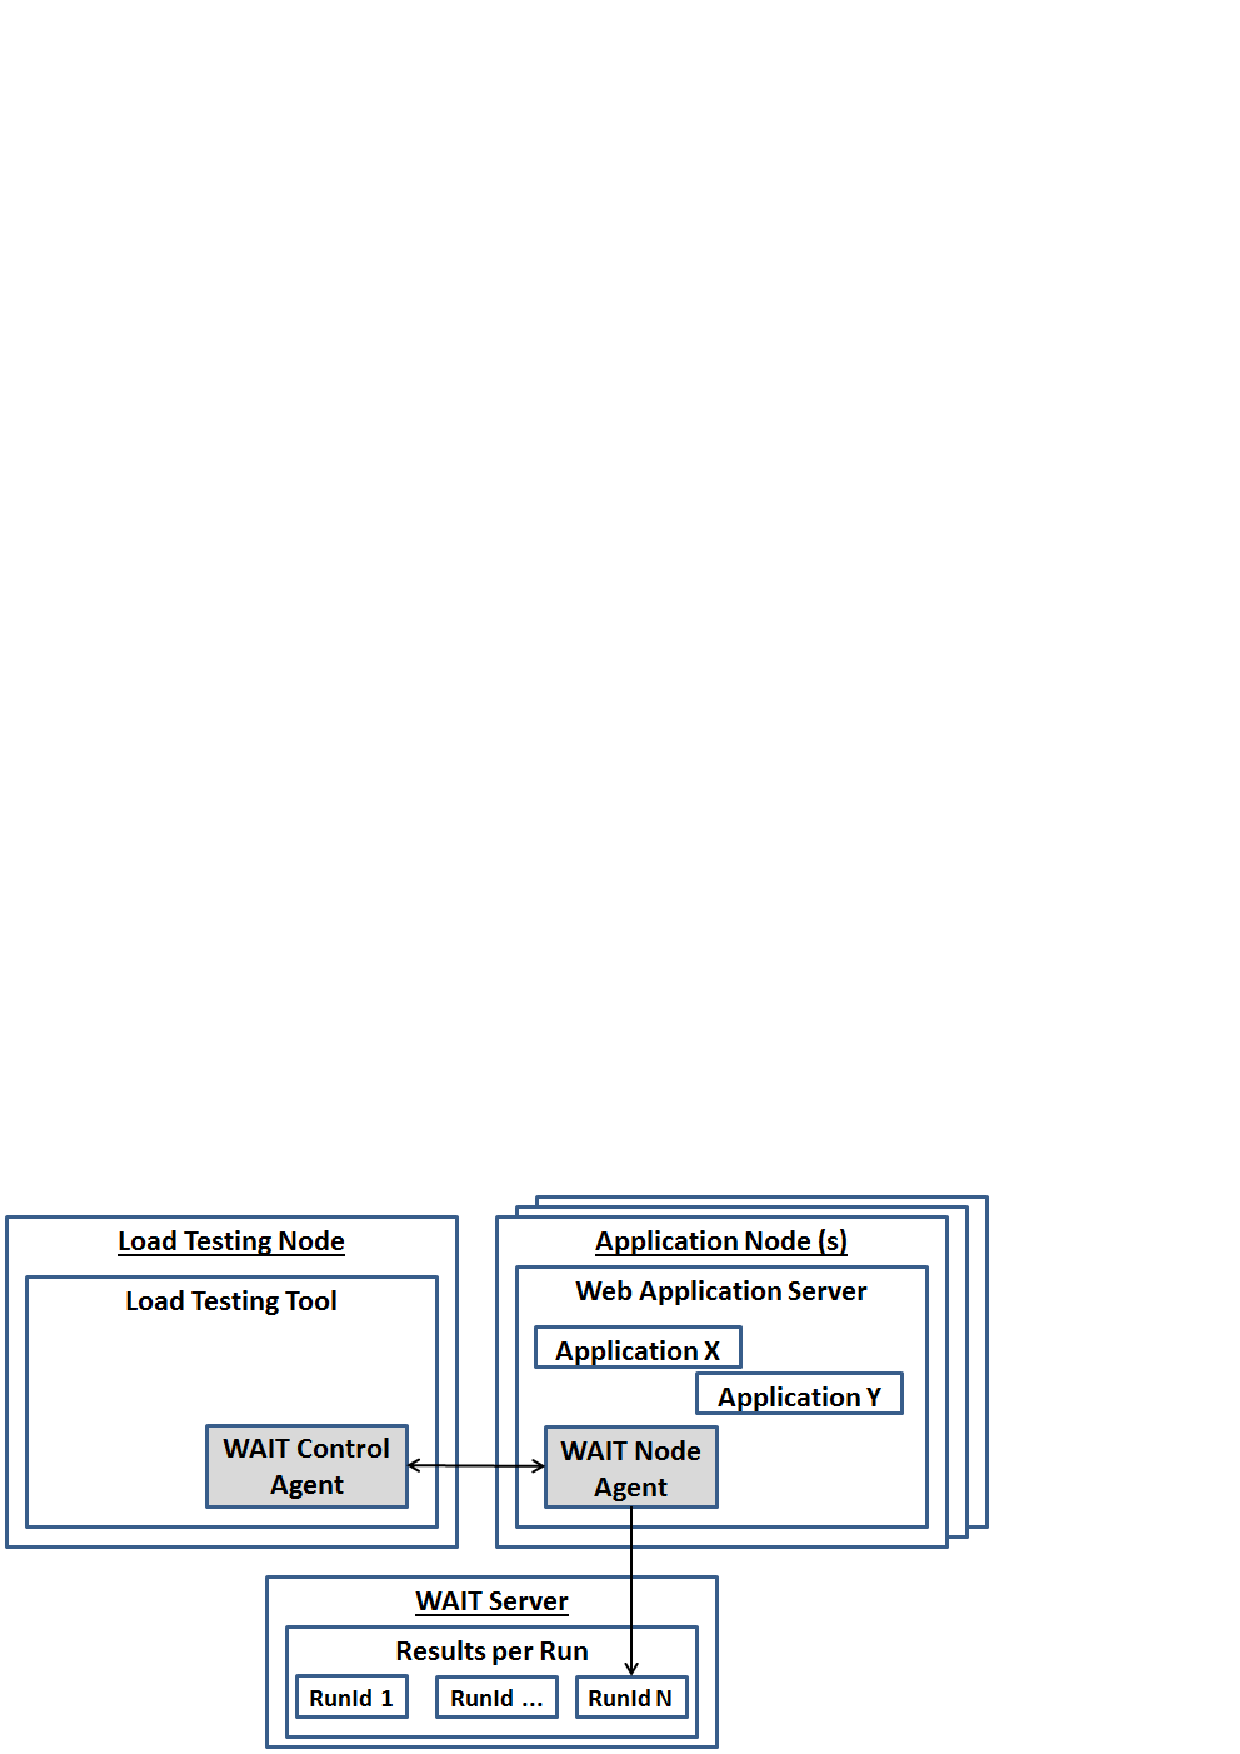
\includegraphics[totalheight=.3\textheight,width=0.9\textwidth]{architecture_dwait}
\caption{High-level Architecture of the solution}
\label{fig_Arch}
\end{figure}

It is important to highlight two assumptions that were considered when defining
the above design. As the scope of this work is the performance testing domain,
it is assumed that a Load Testing tool will always be present in the
testing environment. From the time been, the scope of this work is also focused
on Web Applications (a traditional Java business niche which is also type of 
applications that our industrial partner tests). For this reason, it is also
assumed at this stage that there will always be a Web Application Server in each
one of the application nodes. This assumption has the extra benefit that the
\emph{WAIT Node Agent} is a Web Application. As it uses plain HTTP protocol
to interact with the \emph{WAIT Control Agent}, a single version of \emph{WAIT
Node Agent} could interact with multiples types of \emph{WAIT Control Agent}
(as it is possibly necessary to have one per type of Load Testing Tool) or even
used independently.

Based on the concepts presented here, a prototype has been developed in
conjunction with our industrial partner IBM. The \emph{WAIT Control Agent} was
implemented as a Eclipse Plugin for the Rational Performance Tester (RPT)
\footnote{http://www-03.ibm.com/software/products/us/en/performance},
while the \emph{WAIT Control Agent} was implemented as a Java Web Application,
composed of a single servlet and a few utility classes. Internally, the
application reuses the data gathering scripts that are currently available for
WAIT \footnote{https://wait.ibm.com/\#page=dataCollectors}. In both cases,
one of the main reason to chose that technology (Eclipse Plugin and Web
Application) was that they are simple to install, as one of the main drivers of
this work is to reduce the testing effort.

Once installed, WAIT can now be configured as any other resource in RPT. This
scenario is shown in \figurename ~\ref{fig_config}. Similarly, once the performance
test has started, WAIT can now be monitored as any other resource in the
\emph{Performance Report} of RPT under the \emph{Resource View}. This is shown
in the \figurename ~\ref{fig_mon}. Finally, the WAIT report (which is initially created 
once the first upload is received and then updated after every data
upload) is also accessible within RPT, so that the tester does not need to
leave RPT during the whole duration of the performance test. This is shown
in \figurename ~\ref{fig_report}.

\begin{figure}[!h]
\centering
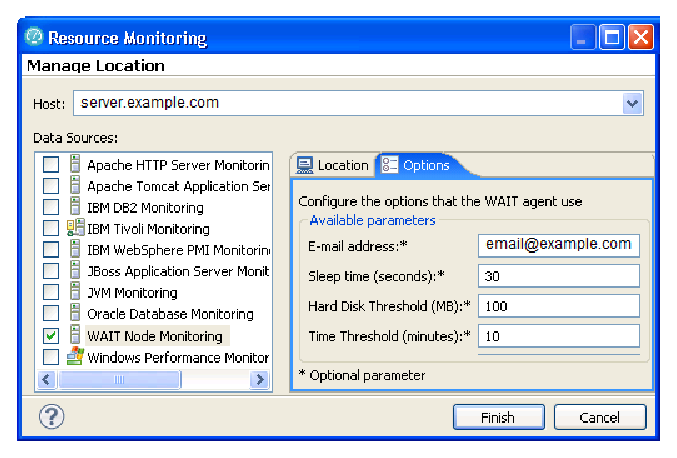
\includegraphics[totalheight=.3\textheight,width=0.8\textwidth]{WAIT-config}
\caption{WAIT configuration through RPT GUI}
\label{fig_config}
\end{figure}

\begin{figure}[!h]
\centering
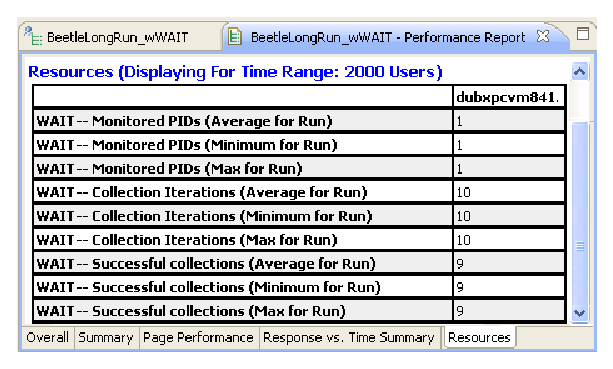
\includegraphics[totalheight=.3\textheight,width=0.8\textwidth]{WAIT-monitoring}
\caption{Monitoring of WAIT Node Agents through RPT}
\label{fig_mon}
\end{figure}

\begin{figure}[!h]
\centering
\includegraphics[totalheight=.4\textheight,width=1.0\textwidth]{WAIT-report}
\caption{WAIT Report available within RPT views}
\label{fig_report}
\end{figure}


%%%%%%%%%%%%%%%%%%%%%%%%%%%%%%%%%%%%%%%%%%%%%%%%%%%%%%%%%%%%%%%%%%%%%%%%%%%%%%%%%%%%%%%%%%%%%%%%%%%%%%%%%%%%
% Experimental Setup / Experiments
%%%%%%%%%%%%%%%%%%%%%%%%%%%%%%%%%%%%%%%%%%%%%%%%%%%%%%%%%%%%%%%%%%%%%%%%%%%%%%%%%%%%%%%%%%%%%%%%%%%%%%%%%%%%

\section{Experimental Evaluation}

In this section the experimental setup is presented along with the experiments themselves. 
After each experiment, its results are also discussed.

In total, 3 experiments were performed. The first two experiments pursed to
answer the research question 2 (How can the overhead be kept low during the whole 
performance test execution to avoid compromising the results?), while the third experiment
pursued to answer the research question 3 (What benefits in productivity can a tester 
achieve if the previous questions are answered?). Finally, the combined outcome
of the three experiments pursued to answer the research question 1 (How can the usage 
of WAIT be automated to minimize the effort required to use it in sync with the performance testing?).

During the evaluation phase 4 different types of nodes were required. An RPT
node, responsible of running the performance test, was a machine running Windows
XP with an Intel Xeon processor at 2.67 Ghz with 3GB of RAM using RPT 8.2.1.3.
A WAIT Server node, where the collected data was uploaded and the results
report was generated, was a machine running Red Hat Enterprise Linux Server 5.9,
with an Intel Xeon processor at 2.66 GHz with 2GB of RAM using Apache Web Server 2.2.3.
One or more application nodes, each one running a 64-bit Windows Server 2008,
with an Intel Xeon E7-8860 (4 cores) at 2.26 GHz with 4GB of RAM and Java 1.6.0
IBM J9 VM (build 2.6). Finally, a Load Balancing node (required in the presence
of multiple application nodes) had the same characteristics of the WAIT Server node using
mod\_jk with a round robin strategy for load balancing purposes.

The above nodes were arranged in 2 environment setups: For the first
experiment, a single application node configuration was used. This environment was composed of one RPT node, 
one application node and one WAIT Server node. For the second and
third experiments, the environment was composed of one RPT node, one load
balance node, two application nodes and one WAIT Server node. Furthermore all
machines are connected by a 10 GBit LAN.These environment set-ups are shown in \figurename ~\ref{fig_env}.

\begin{figure}[!h]
\centering
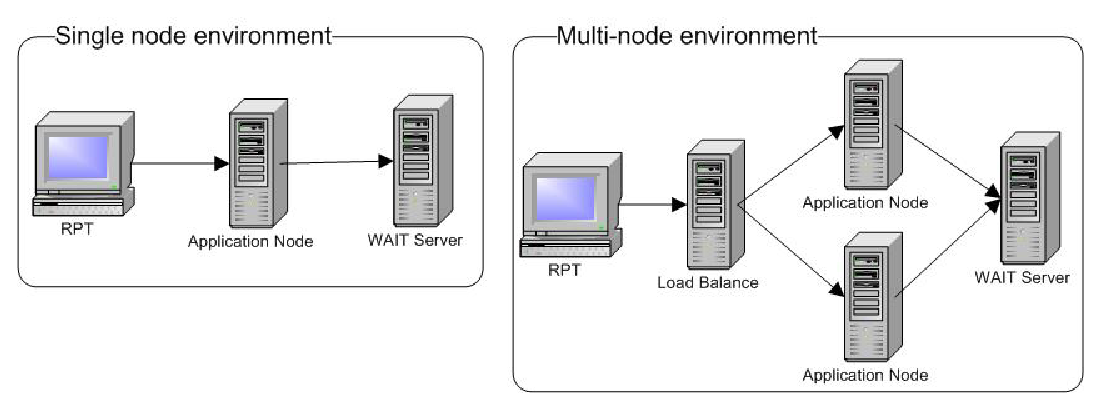
\includegraphics[totalheight=.25\textheight,width=0.8\textwidth]{Environments}
\caption{Environment Set-ups used in the Experiments}
\label{fig_env}
\end{figure}

\subsection{Experiment \#1}

Its objective was to validate that the proposed approach had a low overhead.
It involved the assessment of four metrics: The throughput and response time
(typical metrics used in performance testing) as well as CPU and memory utilization (to assess how much additional resources the automation
requires). All metrics were collected through RPT: RPT directly
calculates throughput and response time, while the resources' utilization was
obtained from the Windows Performance Monitor \footnote{http://technet.microsoft.com/en-us/library/cc768048.aspx} of each application node.

Two real-world applications were selected for this case study. The first
application was iBatis PetStore 4.0
\footnote{http://sourceforge.net/projects/ibatisjpetstore/} which is an 
upgraded version of the Sun's original J2EE Pet Store, a popular e-commerce
shopping cart application used to teach J2EE. This application was run over an Apache
Tomcat 6.0.35 Application Server \footnote{http://tomcat.apache.org/}. The
other application was IBM WebSphere Portal Server 8.0.1
\footnote{http://www-03.ibm.com/software/products/us/en/portalserver},
application which offers enterprise portal capabilities. This application was
run over an IBM WebSphere Application Server 8.0.0.5.
\footnote{http://www-01.ibm.com/software/webservers/appserv/was/}.

This experiment involved two different tests. First, the behaviour of
the approach was tested in a single-node environment to assess how much
overhead it brings under these conditions. For each application, 3 combinations
of WAIT were tried: First the application was executed without WAIT to get a
baseline of how the application performs by itself; then a manual WAIT execution (data collection
scripts directly executed with no upload) was introduced to measure how much
overhead WAIT adds by itself to the application; Finally, the automated approach was introduced to
measure how much overhead it adds. For each of the two combinations that have
WAIT present, two \emph{Sampling Interval} were considered: The first
value was 30 seconds and was selected as a ``worst case" because it is the
minimum value suggested in previous works \cite{Altman2010} to avoid throughput
slowdown above 2\%). The second value was 480 seconds and was selected with the
help of our industrial partner as a representative \emph{Sampling Interval} used in the industry.

All the other parameters involved in the setting up of the performance test
environment were suggested (as per their expert judgment) by our industrial
partner as valid in a realistic test environment: A workload of 2,000 concurrent users; a duration of
1 hour; a \emph{Hard Disk Threshold} of 100MB; a \emph{Time Threshold} of 10
minutes. Finally, for each of the 10 identified combinations (5 per
application), 3 runs were performed. Each run was performed in an unloaded
single-node environment, where the corresponding Web Application Server was restarted 
before every run.

\begin{table}[!h]
\caption{PetStore - Results}
\label{PetStore1}
\centering
\begin{tabular}{p{0.2\textwidth}|p{0.16\textwidth}|p{0.16\textwidth}|p{0.15\textwidth}|p{0.13\textwidth}|p{0.16\textwidth}}
\hline
\bfseries WAIT Modality & \bfseries Avg Response Time (ms)& \bfseries Max
Response Time (ms)& \bfseries Avg Throughput (hps)& \bfseries Avg CPU Usage
(\%) & \bfseries Avg Memory Usage (MB)\\
\hline
None (\emph{Baseline}) 	& 1889.6	& 44704.0	& 158.8 	& 36.9 		& 1429\\
Manual, 480s 			& 0.0\% 	& 0.0\%		& 0.0\%		& 1.1\% 	& 3.0\%\\
Automated, 480s 		& 0.0\%		& 0.0\%		& 0.0\% 	& 2.0\% 	& 3.7\%\\
Manual, 30s 			& 1.6\%		& 0.4\%		& -4.0\% 	& 1.47\% 	& 4.1\%\\
Automated, 30s 			& 4.4\%		& 0.5\%		& -3.1\% 	& 2.53\% 	& 4.4\%\\
%\hline
%Automated, 480s (2 nodes)& 0.5\%	& 0.2\%		& -1.4\% 	& 0.85\% 	& 2.3\%\\
\hline
\end{tabular}
\end{table}

For the PetStore, each performance test produced above 500,000 transactions,
with 99\% of successful transactions. The results showed that using WAIT with a
\emph{Sample Interval} of 480 seconds had practically no impact in terms of response 
time and throughput. Furthermore the difference in resource consumption between
the manual and automated approaches was around 1\%. From a functional perspective, the main 
difference between the two approaches was the presence in the automated one of
the WebAgent and the additional process of uploading and backing up the results. As the 
transferred data is minimal (around 200KB every 10 minutes, mostly composed by
javacores, which are the biggest part of the collected data and with an average size of 1MB 
and ~100KB after compression), the main cause behind the differences in resource
consumption should be the presence of the WebAgent. When WAIT is used with a \emph{Sample Interval} 
of 30 seconds, the impacts in response time and throughput appear. As the impact in throughput is
similar between both approaches, this must have been caused by the javacore
generation (step shared between both approaches). As an average, each javacore took around
1 second to be generated (with a maximum in the worst case scenarios of 1.5
seconds). Even though this cost was neglectable in the higher \emph{Sample
Interval}, with 30 seconds the impact was visible. On the contrary, the difference in response times (2.8\%, approximately 53 milliseconds) was caused by the upload
and backup processes (around 4MB of transferred data), as the cost of the
WebAgent has already been measured in the scenario of a \emph{Sample Interval}.
In terms of resource consumption, the differences between the manual and
automated approach remained very similar to the scenario of a \emph{Sample
Interval} of 480 seconds. The detailed results of these experiments are shown in the \tablename
~\ref{PetStore1} where the first data row shows the results of running the
application alone and the rest the different modalities of WAIT that were
tested.

\begin{table}[!h]
\caption{Portal - Results}
\label{Portal1}
\centering
\begin{tabular}{p{0.2\textwidth}|p{0.16\textwidth}|p{0.16\textwidth}|p{0.15\textwidth}|p{0.13\textwidth}|p{0.16\textwidth}}
\hline
\bfseries WAIT Modality & \bfseries Avg Response Time (ms)& \bfseries Max
Response Time (ms)& \bfseries Avg Throughput (hps)& \bfseries Avg CPU Usage
(\%) & \bfseries Avg Memory Usage (MB)\\
\hline
None (\emph{Baseline}) 	& 4704.75	& 40435.50	& 98.05 	& 76.73 	& 3171.20\\
Manual, 480s 			& 0.7\% 	& 0.6\%		& -0.1\%	& 1.13\% 	& 2.2\%\\
Automated, 480s 		& 3.4\%		& 1.0\%		& -2.8\% 	& 0.63\% 	& 4.1\%\\
Manual, 30s 			& 14.9\%	& 5.4\%		& -5.7\% 	& 2.97\% 	& 5.3\%\\
Automated, 30s 			& 16.8\%	& 9.1\%		& -5.6\% 	& 2.23\% 	& 6.0\%\\
\hline
\end{tabular}
\end{table}

For the Portal, each performance test produced above 400,000 transactions,
with 99\% of successful transactions. Even though the results showed similar
trends (than PetStore) in terms of achieving lower overheads using the
\emph{Sampling Interval} of 480 seconds against the 30 seconds, few key 
differences were identified: First, the impact in response time and
throughput is visible since the \emph{Sampling Interval} of 480 seconds, 
while the impacts are different between using the automated and the manual
approaches. Besides, the differences between using the two \emph{Sampling Intervals} 
are bigger. As the experiment conditions were the same, it was assumed that these 
differences were related to the natural difference in functionality between the
tested applications. This was later confirmed after analyzing the javacores
generated by the Portal, which allowed to measure quantitatively the
differences in behavior of Portal: Its average size was 5.5MB (5.5 times the
average of PetStore's). Moreover its average generation time was 2s (2 times the 
average of PetStore's), with a maximum generation time of 3s (also 2 times the
maximum of PetStore's). The detailed results of these experiments are shown in the \tablename ~\ref{Portal1}.

Due to the relatively small differences between the runs and some variations
(presumable environmental) that were experienced during the execution of the
experiments, it was decided to perform a Paired t-Test
\footnote{http://www.aspfree.com/c/a/braindump/comparing-data-sets-using-statistical-analysis-in-excel/}
to evaluate if the data sets of response time and throughput were significantly
different from each other (using a significant level of p<0.1). The results
showed that for the PetStore application the differences were only significant for
those runs using the \emph{Sample Interval} of 30 seconds in the average
response time, and only for the automated approach using the \emph{Sample
Interval} of 30 seconds in the average throughput. In the case of Portal, the
results were similar. This additional analysis reinforced the
previous observation that it is preferable, in terms of overhead, the
usage of the \emph{Sample Interval} of 480 seconds. The detailed results of
this analysis are shown in the \tablename ~\ref{tTest1}.

 [PENDING: Rephrase t-test results using feedback from Philip]

\begin{table}[!h]
\caption{t-Test - Probability Results}
\label{tTest1}
\centering
\begin{tabular}{p{0.2\textwidth}|p{0.2\textwidth}|p{0.2\textwidth}|p{0.2\textwidth}|p{0.2\textwidth}}
\hline
\bfseries Application & \bfseries WAIT Modality & \bfseries Avg Response Time
(ms)& \bfseries Max Response Time (ms)& \bfseries Avg Throughput (hps)\\
\hline
PetStore & 	Manual, 480s 			& 0.470 & 0.143	& 0.206\\
PetStore & 	Automated, 480s 		& 0.342	& 0.297	& 0.472\\
PetStore & 	Manual, 30s 			& 0.089	& 0.241	& 0.154\\
PetStore & 	Automated, 30s 			& 0.019	& 0.334	& 0.078\\
\hline
Portal 	& 	Manual, 480s 			& 0.140 & 0.263	& 0.496\\
Portal 	& 	Automated, 480s 		& 0.040	& 0.189	& 0.131\\
Portal 	& 	Manual, 30s 			& 0.001	& 0.158	& 0.167\\
Portal 	& 	Automated, 30s 			& 0.013	& 0.105	& 0.072\\
\hline
\end{tabular}
\end{table}

A second test was performed with the objective of validating that the proposed
approach was reliable and its overhead remained low in a multi-node environment
and during a longer test run. The iBatis PetStore 4.0 application was selected for 
this test due to the available of an environment to test it as well as the
availability of its source code (required for the experiment \#2). Based on the 
finding of the previous test, only two 2 WAIT combinations were tested: First
the application was executed alone to have a baseline of how it performs by itself; 
then the automated WAIT approach was introduced to measure its overhead, using the 
\emph{Sampling Interval} of 480 seconds, which not only the one suggested by
the performance testing team of our industrial partner but also the best 
performer from the previous test. All the other parameters involved in the
setting up of the performance test were identical to the first experiment with 
two exemptions: The workload was doubled to compensate for the additional
application node and the selected duration was 24 hours. Finally, each run was performed 
in an unloaded multi-node environment, where all components were restarted
before every run.

Even though the results were slightly different than the single-node run,
they proved the the solution is reliable, as using WAIT with a
\emph{Sample Interval} of 480 seconds during the 24-hour runs had minimal impact
(up to 1.4\%) in terms of response time and throughput. Similarly, the
consumption of resources behaved similarly (up to 2.3\%). The detailed results of 
these experiments are shown in the \tablename ~\ref{Portal2}. Finally, a
Paired t-Test was performed and it confirmed that the differences between the
runs were not statistically significant.

\begin{table}[!h]
\caption{Multi-node PetStore - results}
\label{Portal2}
\centering
\begin{tabular}{p{0.2\textwidth}|p{0.16\textwidth}|p{0.16\textwidth}|p{0.15\textwidth}|p{0.13\textwidth}|p{0.16\textwidth}}
\hline
\bfseries WAIT Modality & \bfseries Avg Response Time (ms)& \bfseries Max
Response Time (ms)& \bfseries Avg Throughput (hps)& \bfseries Avg CPU Usage
(\%) & \bfseries Avg Memory Usage (MB)\\
\hline
None (\emph{Baseline}) 	& 2669.62	& 47346.10	& 157.68 	& 45.27 	& 1831.10\\
Automated, 480s 		& 0.5\%		& 0.2\%		& -1.4\% 	& 0.85\% 	& 2.3\%\\
\hline
\end{tabular}
\end{table}

In conclusion, the results of this first experiment showed that the overheads
caused by the automated approach can be kept low during the whole performance
test execution. This answer our research question Q2 positively, only with a side
note: Due to the impact the \emph{Sampling Interval} and the application
behavior could have in the overhead, it is important to keep this in mind when
using WAIT. For example, the \emph{Sampling Interval} of 480 seconds
proved efficient in terms of overhead for the two tested applications.

\subsection{Experiment \#2}

The objective of this second experiment was to assess the benefits the approach
brings to a performance tester. For this experiment the automated approach was
configured to monitor a modified version of the iBatis PetStore 4.0 application.
The source code of this application was modified to inject some performance
issues to assess how WAIT was able to identify them and estimate the corresponding 
time savings in performance analysis. Specifically, 3 common performance issues were 
injected: A lock contention bug, composed by a very heavy calculation within a
synchronized block of code; a I/O latency bug, composed by a very expensive file reading 
method; and a deadlock bug, in particular an implementation of the classic
``friends bowing'' deadlock example
\footnote{http://docs.oracle.com/javase/tutorial/essential/concurrency/deadlock.html}.
All other parameters involved in the setting up of the performance test were
identical to the multi-node test performed in the previous experiment with
exception of the test duration which was 1-hour. Finally, only the most relevant
sections of the GUI for each issue are presented in order to save space.

Surprisingly the first ranked issue was none of the injected bugs but
a method call named ``McastServiceImpl.receive'' which appeared in practically all
the threads. It was a unexpected finding which lead to some extra analysis
to determine it was benigne, as these method invocations are part of the
clustering functionality of Tomcat. The secondly ranked issue was the lock
contention. A relevant point to notice is that these two issues were
detected since the first version of the report (generated at minute 10, right
after the first data collection phase occurred). Based on the high recurrency of
the issues (above 96\% of the samples in both cases), this information could
have let the testers to raise bugs and pass this information to the development
team so that the diagnosis could start far ahead of the test completion. Talking a
look to the final version of the report reinforced the presence of these issues
by offering similar ranks. These additional information could also be documented
and shared with the development team about the relevance of the issues.
\figurename ~\ref{fig_run1_bugs12}.a shows the results of the first generated report, 
while ~\ref{fig_run1_bugs12}.b shows the results of the final report.

\begin{figure}[!h]
% \centering
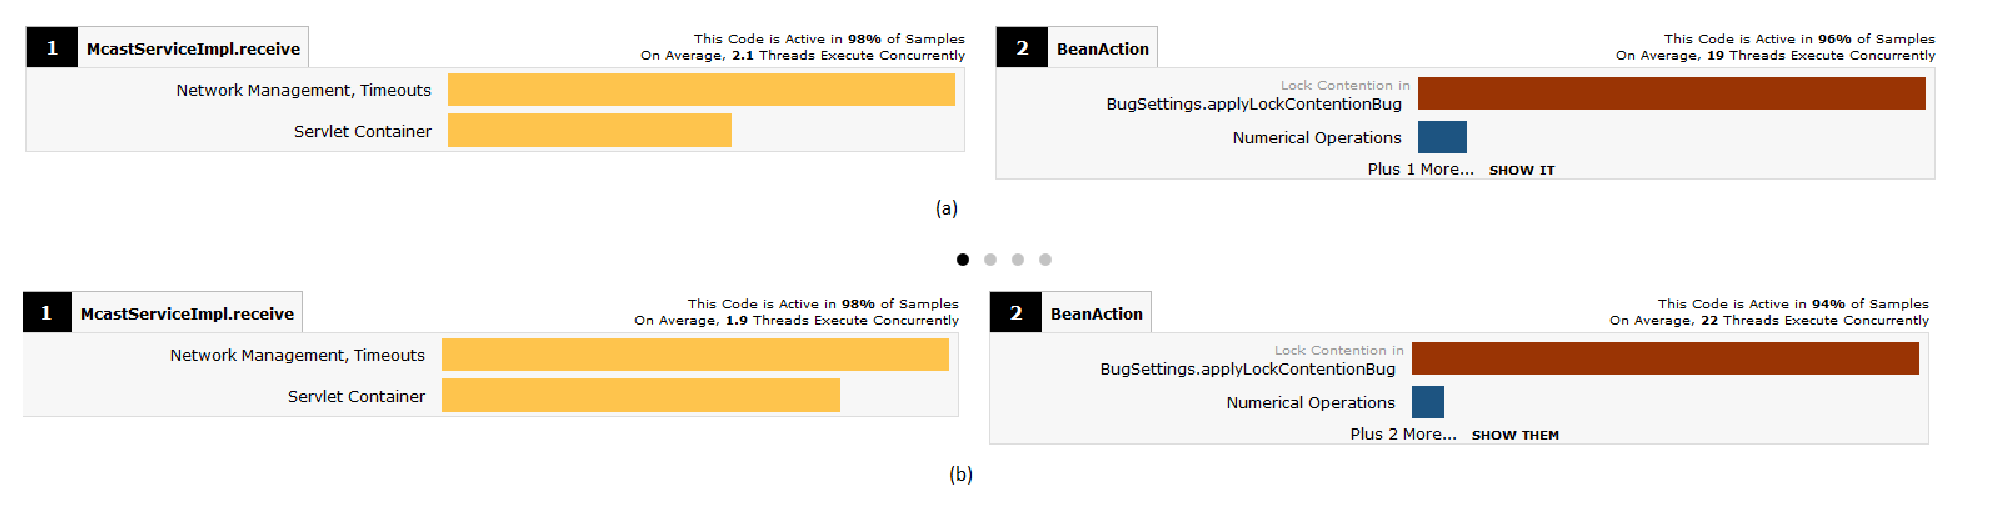
\includegraphics[totalheight=.25\textheight,width=1\textwidth]{run1_issues12_short_long_run}
\caption{Top detected performance issues in modified JPetStore application}
\label{fig_run1_bugs12}
\end{figure}

After identifying a performance issue, one can go one level down to see more
details about the detected issue, such as the type of problem, involved class, method and method line. 
\figurename ~\ref{fig_issue2_vs_code} shows the information of our Lock
Contention bug, which was located in the LockContentionBug class, method
generateBug, line 20. When comparing it with the actual source code, one can
see that is precisely the line where the bug was injected (by taking a class
lock and then doing a very CPU intensive logic - the calculation of Pi using
BigDecimal classes -).

\begin{figure}[!h]
% \centering
\includegraphics[totalheight=.3\textheight,width=1\textwidth]{issue2_vs_code}
\caption{Comparison of lock contention issue in the WAIT report against the
actual source code}
\label{fig_issue2_vs_code}
\end{figure}

The report showed in 3rd place another symptom of the lock contention issue
(it was able to relate the issues by comparing their detail information, where
both issues pinpointed to the same class/method). This additional evidence
suggested that this was definetely a major issue in the application. Moreover
the I/O latency bug was also identified by this test run, ranking it in 4th
place of severity. An interesting finding was that the deadlock issue did not
present in this run, most likely prevented by the fact that the injected lock
contention bug had a major impact in the application that originally planned.
\figurename ~\ref{fig_issues34} shows the details of these two issues.

\begin{figure}[!h]
% \centering
\includegraphics[totalheight=.3\textheight,width=1\textwidth]{run1_issues34_details}
\caption{Details of issues ranked 3 and 4 in the first test run}
\label{fig_issues34}
\end{figure}

Based on the obtained information, the two identified bugs were ``corrected''
and removed from the source code. Emulating a common test cycle, another run
was done to see if there was any remaining performance issues in the
application. Not surprisingly, the deadlock bug did appear in this report and,
similarly to the previous cases, the report information, complemented
with its comparison against the source code allowed the issue identification.
A point worth noticing is that, even though the presence of the issue was
correctly identified by WAIT, in this particular case it was not able to
categorize it (leaving it with a blank color). \figurename
~\ref{fig_dlissue_vs_code} shows the information of our Deadlock bug, which was
located in the Friend private class within the DeadLockBug class, in the line
30 of the method bow. When comparing it with the actual source code, one can
see that is precisely the line where the bug was injected (as the deadlock logic 
implemented the classing example of the bowing friends, the actual deadlock
occurred when friends try to bowBack to each other).

\begin{figure}[!h]
% \centering
\includegraphics[totalheight=.3\textheight,width=1\textwidth]{deadlock_vs_code}
\caption{Comparison of deadlock issue in the WAIT report against the
actual source code}
\label{fig_dlissue_vs_code}
\end{figure}

As the main measurement of success for this experiment was to assess the
ability of WAIT to identify performance problems, this experiment was
successful as all three injected bugs were identified, including the
involved classes and methods. 

In terms of time, two main savings were identified. First, the automated
approach practically reduced the overhead of collecting data for WAIT (which
previously was too high and practically made WAIT unusable in a highly
distributed environment) to zero. In parallel to the execution of all the performed 
experiments (around 40 performance tests, for an approximated combined test
duration of 60 hours), the time spent in using of WAIT was tracked. The total 
installation time of the automated approach (Eclipse plugin and WebAgent) took
no more than 15 minutes. After that, its usage require practically no additional time over the regular usage of the
RPT (barely a minute, or less, to change its settings whenever needed -i.e. to
modify the \emph{Sampling Interval}- or enabling/disabling its usage -i.e. to
switch back and forth between the manual and automated modes-).

The second time saving was in terms of reducing the effort invested
in performance analysis. Even though the amount of injected bugs was
small, the results would allow to estimate the potential benefits. Previously, 
a tester would have ended with multiple WAIT reports (assuming he was able to
collect the required information with the desired upload frequency). For
example, assuming a distributed environment composed of X nodes, with a desired
time window of 1-hour and a test duration of Y hours, a tester would end with X*Y 
different WAIT reports, having to review X reports every hour (which means a
number of reports directly proportional to the number of monitored nodes). With
the automated approach, a tester should only have to review a single report,
regardless of the number of nodes that compose the environment, which get refreshed 
every hour.

[PENDING: Modify to include/stress that the assumption of a single node would
not work, as the workload might be different between nodes. For example, it is
common that load test use different distributions to emulate different
customer behaviors, which might involve testing different transactions among
the application nodes.]

Furthermore, overcoming the usability constraints of WAIT allow a tester
to enjoy the natural benefits of WAIT and exploit its expert knowledge
capabilities\footnote{https://wait.ibm.com/waitUserManual.pdf} to expedite the
identification of performance issues and its root causes. Even though it
might be hard to define an average time spent identifying performance issues,
even a conservative estimate (i.e. a couple of hours) could help to
quantify WAIT's savings. For example in our study case, instead of spending 6
hours analyzing the issues, it was possible to identifying them and the involved
source code only with the information provided by the WAIT report. Moreover
the automated approach would allow a wider range of testers to do performance
analysis activities. An additional benefit is that less experienced testers
could use this information to gain a deeper understanding of these type of problems, 
hence reducing the dependency and overall workload of the most expert users
within a team.

Finally, as the report is updated on a recurrent basis, a tester does
not need to wait until the end of the test to assess the results and raise bugs
if required. As seen in the above experiment, additional time can be saved
in the test process by reporting any relevant issue in parallel to the
execution of the test, allowing the development team to start working on it.
This would be especially valuable in long-term runs which are very common in the 
performance testing domain, usually lasting several days.

In conclusion, the results of this second experiment answered our research
question Q3 (What benefits in productivity can a tester achieve if the previous
two questions are answered?), by showing those productivity gains that a tester
achieves by using the automated approach of WAIT.

To summarize the overall experimental results, they were satisfactory because it
was possible to achieve the desired goals of automating the execution of WAIT,
while keeping the overhead low (in the range of 0\% to 3\% using a \emph{Sample
Interval} of 480 seconds). Furthermore it was possible to assess the time
savings the automated approach brings to the test process: After a quick
installation effort (around 5 minutes per node), the time required by a tester
to use WAIT as part of a performance testing is practically zero. Previously the
number of WAIT reports that a tester needed to review was equal to the number of
nodes of the tested environment (which in a highly distributed environment
might be hundreds or more) multiplied by the number of times the collected
information was uploaded (in order to have an incremental view); now, only
a tester only needs to monitor a single report, which is updated on a recurrent
basis to offer an incremental view of the results. A direct benefit of these
savings is the reduction of expert knowledge required by tester in order to do
performance analysis and be able to detect the performance issues and their
root causes. Ultimately, this improves the tester productivity by reducing the
cost (in terms of effort) required to locate defects.


\subsection{Threads to Validity}

Like any empirical work, there are a number of threats to the validity of these
experiments. The first one is the potential environmental noise could affect in
the testing environments considering that the environments are not isolated. To
mitigate the potential effect the noise might have in the obtained results, multiple runs 
were executed for each identified combination. Additionally, in order to know if
the differences between the obtained results were statistically significant (specially in cases 
were the differences were minimal, for example between the runs of the
applications alone against those runs using WAIT with a very low sample rate), the statistic Paired t-Test
\footnote{http://www.aspfree.com/c/a/braindump/comparing-data-sets-using-statistical-analysis-in-excel/}
was performed to determine if the null hypothesis (the changes in the
environment, practically the addition of WAIT in different forms, have no
impact in the environment) was rejected or not with 95\% of certainty.

Another thread is the selection of the performance testing parameters (i.e.
workload and duration of the test). This was addressed with the expert judgement 
of the SVT, which couched on the selection of those parameters that are
commonly used in the industry. Finally, the validity of these results are
threatened by the selection of the tested applications. Despite the fact that
they are real world applications and different in terms of functionality, their
limited number implies that not all types of applications have been tested and
one application with characteristics that are completely different might
generate different results. Wider experiments need to be executed to get more
general conclusions. However, in principle, there is no reason to believe that
the approach is not applicable to other environments.


%%%%%%%%%%%%%%%%%%%%%%%%%%%%%%%%%%%%%%%%%%%%%%%%%%%%%%%%%%%%%%%%%%%%%%%%%%%%%%%%%%%%%%%%%%%%%%%%%%%%%%%%%%%%
% Section 7: Conclusions
%%%%%%%%%%%%%%%%%%%%%%%%%%%%%%%%%%%%%%%%%%%%%%%%%%%%%%%%%%%%%%%%%%%%%%%%%%%%%%%%%%%%%%%%%%%%%%%%%%%%%%%%%%%%

\section{Conclusions and Future Work}

The identification of performance problems and the diagnosis of their root
causes are very complex and time-consuming activities in highly distributed
environments, which also tend to rely on the expertise of the involved
engineers. The objective of this work was to address the limitations that
prevent the usage of WAIT in the performance testing domain, so that WAIT can be
effective used to reduce the expertise and overall effort required to do
good performance analysis and to identify the root causes of those issues.
To achieve this goal the paper presented a novel automation approach and its
validation, composed of the implementation of a prototype and a study
case with two real-life applications. The results are encouraging as they have
proved that the approach addresses effectively the adoption barriers for WAIT in 
a distributed performance testing environment: The solution has proven being
light-weight, generating a low overhead ([PENDING]). Moreover, from a tester
usability perspective, there are also tangible time savings in terms of the
effort required to detect performance issues.

Future work will concentrate on assessing the practicability of the
approach and its benefits in a major scale through broader study cases with our
industrial partner IBM. It will also be evaluated how best to exploit the
additional functional information that can now be obtained from a tested environment
(i.e. test workload, response time, throughput and transactions) in order to
improve the qualitative and quantitative capabilities of the idle-time
analysis methodology (over which WAIT is based on) to identify more
types of performance problems.
[PENDING: Also to deepen the analysis in the relationship between the nature of
the application - represented by the javacore size and its contents - and the
sampling interval]

%%%%%%%%%%%%%%%%%%%%%%%%%%%%%%%%%%%%%%%%%%%%%%%%%%%%%%%%%%%%%%%%%%%%%%%%%%%%%%%%%%%%%%%%%%%%%%%%%%%%%%%%%%%%
% Section 8: Acknowledgements
%%%%%%%%%%%%%%%%%%%%%%%%%%%%%%%%%%%%%%%%%%%%%%%%%%%%%%%%%%%%%%%%%%%%%%%%%%%%%%%%%%%%%%%%%%%%%%%%%%%%%%%%%%%%

\section*{Acknowledgments}

We would like to thanks Amarendra Darisa, from SVT IBM Dublin, as his expertise
and experience in performance testing helped us through the scope definition and validation of this work.

This work was supported, in part, by Science Foundation Ireland grant 10/CE/I1855 to Lero - the Irish Software Engineering Research Centre (www.lero.ie).

% Between 12 - 24 \ldots 18 sounds like a good number!
\bibliographystyle{splncs}
\bibliography{dwait_manual,dwait}

%\section*{Appendix: Springer-Author Discount}

\end{document}

The idea of applying automation in the performance testing domain is not new.
However most of the existing performance testing research has focused on
automating the generation of load test suites \cite{Chen1,Elvira1,Zhang1,Briand1,Avritzer1,Bayan1,Avritzer2,Avritzer3,Garousi1}.
Similarly, there are in the industry a variety of commercial products and free open-source tools 
available to support this task. For example, the HP LoadRunner
\footnote{http://www8.hp.com/us/en/software/
software-product.html?compURI=tcm:245-935779} and the IBM's Rational Performance
Tester \footnote{http://www-01.ibm.com/software/awdtools/tester/performance/} are solutions that allow 
scalability testing by generating a real workload on the application. From the
open-source community, Apache's JMeter \footnote{http://jmeter.apache.org/} and Grinder
\footnote{http://grinder.sourceforge.net/} are two popular applications that provide similar functionality.

Regarding the performance analysis area, it also remains an active research
venue. However, a high percentage of those techniques are not suitable to the
performance testing domain because have an impractical performance overhead.
For example, the authors of \cite{Yang1} instrument the source code to mine
the sequences of call graphs and infer, through the usage of heuristics, the relevant 
error patterns. In addition to the instrumentation, which generates a high
performance overhead, this approach requires a considerable manual effort.

Similar case of the work presented in \cite{Hangal1,Csallner1} which use
dynamically inferred invariants to detect programming errors or the work
proposed by \cite{Barham1,Chen2} which are also performance analysis approaches
based on instrumentation. In all cases, these techniques cannot be
effectively applied to load testing due to the impractical performance overhead
that the instrumentation would bring to the tested environments. The main
difference between these approaches and ours is that no instrumentation of the
monitored system is required, eliminating a major source of potential overhead.

One of the closest works to ours is \cite{Jiang2009}. In this paper, the authors
present a non-intrusive approach which automatically analyzes the execution logs
of a load test in order to identify performance problems. This approach requires to have
information from a previous run to use it as baseline, information which might
not be available in all the cases. As this approach only uses 
the load testing results (i.e. response time and throughput) in its analysis,
the deepness of its analysis in terms of root causes is limited, as it cannot offer 
hints about what is causing the performance issues that identifies. 

[PENDING: To rephrase this part!]

On the contrary, 
To the best of our knowledge, our approach is the first to propose the
applicability, through automation means, of the idle-time analysis in the performance testing domain to exploit its performance analysis capabilities.

being the first of its type, to the best of our knowledge.

[PENDING: Should I bring back the pseudo-motivation of expert -maybe
automation efforts to reduce the expert knowledge required to do performance
testing/analysis:  (i.e. RTCE, GC Lite, LeakChaser), runtime vs. static. Some
similar, but different in the sources they use and the domain?-]

----------------------------
  
  PENDING:
  - Complete the related work sections!
  - Re-read the paper to see if it makes sense (i.e. the verbiage of the
  reserch questions should change to make a better fit with the experiments
  and their results).

[PENDING: Should I add any mention of the sanity check? (about HD) probably
only if suggested]
 
 [PENDING:
 
 Probably improve the verbiage related to JPetStore to something like this:
 
 JPetStore [2] is a larger and more complex open source web application relative
 to DS2. Unlike Sun’s original ver- sion of Pet Store which is more focused on demonstrat- 
 ing the capability of the J2EE platform, JPetStore is a re- implementation with a more efficient 
 design [3] and is tar- geted on benchmarking the J2EE platform against other web platforms such as 
 .Net. Unlike DS2 which embeds all the application logic into the JSP code, JPetStore uses the 
 “Model-View-Controller” framework andXMLfiles for ob- ject/relational mappings. In this task, 
 we have deployed the JPetStore application on Apache Tomcat and used MySQL as the database backend. 
 ]
  